%-------------------------
% Resume in Latex
% Author : Pau Bover Femenias
% As MIT Template
% Based on Harshibar's work
%------------------------

\documentclass[letterpaper,11pt]{article}

\usepackage{latexsym}
\usepackage[empty]{fullpage}
\usepackage{titlesec}
\usepackage{marvosym}
\usepackage[usenames,dvipsnames]{color}
\usepackage{verbatim}
\usepackage{enumitem}
\usepackage[hidelinks]{hyperref}
\usepackage{fancyhdr}
\usepackage[english]{babel}
\usepackage{tabularx}
\usepackage{graphicx}
% only for pdflatex
% \input{glyphtounicode}

% fontawesome
\usepackage{fontawesome5}

% fixed width
\usepackage[scale=0.90,lf]{FiraMono}

% light-grey
\definecolor{light-grey}{gray}{0.83}
\definecolor{dark-grey}{gray}{0.3}
\definecolor{text-grey}{gray}{.08}

\DeclareRobustCommand{\ebseries}{\fontseries{eb}\selectfont}
\DeclareTextFontCommand{\texteb}{\ebseries}

% custom underilne
\usepackage{contour}
\usepackage[normalem]{ulem}
\renewcommand{\ULdepth}{1.8pt}
\contourlength{0.8pt}
\newcommand{\myuline}[1]{%
  \uline{\phantom{#1}}%
  \llap{\contour{white}{#1}}%
}


% custom font: helvetica-style
\usepackage{tgheros}
\renewcommand*\familydefault{\sfdefault} 
%% Only if the base font of the document is to be sans serif
\usepackage[T1]{fontenc}


\pagestyle{fancy}
\fancyhf{} % clear all header and footer fields
\fancyfoot{}
\renewcommand{\headrulewidth}{0pt}
\renewcommand{\footrulewidth}{0pt}

% Adjust margins
\addtolength{\oddsidemargin}{-0.5in}
\addtolength{\evensidemargin}{0in}
\addtolength{\textwidth}{1in}
\addtolength{\topmargin}{-.5in}
\addtolength{\textheight}{1.0in}

\urlstyle{same}

\raggedbottom
\raggedright
\setlength{\tabcolsep}{0in}

% Sections formatting - serif
% \titleformat{\section}{
%   \vspace{2pt} \scshape \raggedright\large % header section
% }{}{0em}{}[\color{black} \titlerule \vspace{-5pt}]

% TODO EBSERIES
% sans serif sections
\titleformat {\section}{
    \bfseries \vspace{2pt} \raggedright \large % header section
}{}{0em}{}[\color{light-grey} {\titlerule[2pt]} \vspace{-4pt}]

% only for pdflatex
% Ensure that generate pdf is machine readable/ATS parsable
% \pdfgentounicode=1

%-------------------------
% Custom commands
\newcommand{\resumeItem}[1]{
  \item\small{
    {#1 \vspace{-1pt}}
  }
}

\newcommand{\resumeSubheading}[4]{
  \vspace{-1pt}\item
    \begin{tabular*}{\textwidth}[t]{l@{\extracolsep{\fill}}r}
      \textbf{#1} & {\color{dark-grey}\small #2}\vspace{1pt}\\ % top row of resume entry
      \textit{#3} & {\color{dark-grey} \small #4}\\ % second row of resume entry
    \end{tabular*}\vspace{-4pt}
}

\newcommand{\resumeSubSubheading}[2]{
    \item
    \begin{tabular*}{\textwidth}{l@{\extracolsep{\fill}}r}
      \textit{\small#1} & \textit{\small #2} \\
    \end{tabular*}\vspace{-7pt}
}

\newcommand{\resumeProjectHeading}[2]{
    \item
    \begin{tabular*}{\textwidth}{l@{\extracolsep{\fill}}r}
      #1 & {\small\color{dark-grey} #2} \\
    \end{tabular*}\vspace{-1pt}
}

\newcommand{\resumeSubItem}[1]{\resumeItem{#1}\vspace{-4pt}}

\renewcommand\labelitemii{$\vcenter{\hbox{\tiny$\bullet$}}$}

% CHANGED default leftmargin  0.15 in
\newcommand{\resumeSubHeadingListStart}{\begin{itemize}[leftmargin=0in, label={}]}
\newcommand{\resumeSubHeadingListEnd}{\end{itemize}}
\newcommand{\resumeItemListStart}{\begin{itemize}[leftmargin=*, itemsep=4pt]}
\newcommand{\resumeItemListEnd}{\end{itemize} \vspace{1pt}}

\color{text-grey}

%-------------------------------------------
%%%%%%  RESUME STARTS HERE  %%%%%%%%%%%%%%%%%%%%%%%%%%%%


\begin{document}

%----------HEADING----------

\begin{tabular*}{\textwidth}{@{}l@{\extracolsep{\fill}}r@{}}

\begin{minipage}[c]{0.72\textwidth}
{\Huge \textbf{Pau Bover Femenias}} \\[6pt]

\small
\faPhone* \hspace{4pt} +xx xxx xxx xxx \hspace{8pt} $|$ \hspace{8pt}  
\faEnvelope \hspace{4pt} xxxxxxxxxx@gmail.com \\[2pt]

\faGithub \hspace{4pt} BoverPau333 \hspace{8pt} $|$
\faLinkedin \hspace{8pt} BoverPau333 \hspace{8pt} $|$  \hspace{8pt}
\faMapMarker* \hspace{4pt} Palma de Mallorca, Spain

\end{minipage}
&
\begin{minipage}[c]{0.22\textwidth}
\raggedleft
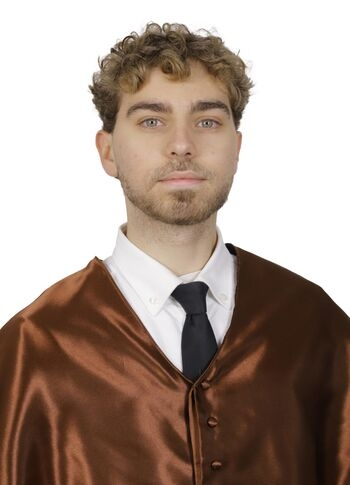
\includegraphics[width=3cm]{personalPhoto.jpeg}
\end{minipage}

\end{tabular*}

\vspace{2pt}

%-----------EXPERIENCE-----------
\section{EXPERIENCE}
  \resumeSubHeadingListStart

    \resumeSubheading
    {BehindThePixel}{Jun. 2024 -- Present}
    {Technical Project Lead \& Full-Stack Developer}{Palma, Spain / Barcelona, Spain}
            \resumeItemListStart
            \resumeItem{Led a technology-focused SME delivering software solutions across media, AI and digital platforms}
            \resumeItem{Managed client relationships and project requirements while coordinating the full software development lifecycle}
            \resumeItem{Designed and developed full-stack architectures and scalable systems for web platforms and automated services}
            \resumeItem{Designed and implemented \textbf{AI-driven systems} for automated content programming and recommendation}
            \resumeItem{\textbf{Clients:} Musicalitat, Producions Blau, Vibra Hotels, Unió de Consells Esportius de Catalunya, Lottusse, Discmedi, Govern de les illes Balears among others}
    \resumeItemListEnd

    \resumeSubheading
    {NTT DATA}{Feb. 2026 -- Jun. 2026}
    {Backend Developer Intern}{Granada, Spain}
        \resumeItemListStart
        \resumeItem{Worked as a backend development intern contributing to enterprise software solutions for the \textbf{BBVA} client}
        \resumeItem{Developed and maintained backend services and APIs for internal banking platforms}
        \resumeItem{Collaborated with senior developers and multidisciplinary teams following \textbf{Agile methodologies}}
    \resumeItemListEnd

\resumeSubHeadingListEnd

%-----------PROJECTS-----------

\section{PROJECTS}
\resumeSubHeadingListStart


\resumeProjectHeading
{\textbf{AI-Driven Autonomous Radio Platform}}
{Industry Client Project | 2025}
\resumeItemListStart
\resumeItem{Designed and developed an \textbf{AI-powered radio system} capable of automatically generating music programming based on audience behavior and time-of-day patterns}
\resumeItem{Implemented machine learning models using \textbf{Python and PyTorch} to analyze listening trends and dynamically curate playlists}
\resumeItem{Built the full-stack platform with \textbf{PHP, MySQL and Docker}, enabling autonomous scheduling and real-time content management}
\resumeItem{\textbf{Client:} Musicalitat}
\resumeItemListEnd

\resumeProjectHeading
{\textbf{Online Music Store Platform for Record Labels}}
{Industry Client Project | 2024}
\resumeItemListStart
\resumeItem{Developed a scalable \textbf{full-stack e-commerce platform} for music distribution and merchandising}
\resumeItem{Implemented product catalog management, digital content delivery and payment-ready architecture}
\resumeItem{Designed the database structure and backend services using \textbf{PHP and MySQL}}
\resumeItem{\textbf{Client:} Producions Blau}
\resumeItemListEnd

\resumeProjectHeading
{\textbf{Neural Network Adaptation after Class Modification}}{Bachelor Thesis $|$  2026}
\resumeItemListStart
\resumeItem{Research project focused on \textbf{adapting trained neural networks after class modifications} while minimizing retraining cost}
\resumeItem{Explores techniques related to \textbf{incremental learning, transfer learning and model fine-tuning}}
\resumeItem{Designed experiments to measure \textbf{training efficiency, accuracy preservation and computational cost}}
\resumeItem{Applications in dynamic classification systems where classes evolve over time}
\resumeItemListEnd

\resumeProjectHeading
{\textbf{Red Panda Algorithm Metaheuristic Evaluation}}{Research Project $|$  2026}
\resumeItemListStart
\resumeItem{Conducted a research study analyzing the \textbf{performance of the Red Panda Optimization Algorithm} compared with established metaheuristics}
\resumeItem{Evaluated the algorithm against techniques such as \textbf{Genetic Algorithms  and Local Search among others}}
\resumeItem{Implemented experimental benchmarks using \textbf{C++ and scientific computing libraries}}
\resumeItem{Analyzed convergence speed, solution quality and computational efficiency across multiple dimensions}
\resumeItem{Provided a comparative study highlighting strengths and limitations of the Red Panda metaheuristic in complex search spaces}
\resumeItemListEnd

\resumeProjectHeading
{\textbf{Real-Time Tennis Match Analysis}}{Computer Vision Project $|$ 2025-2026}
\resumeItemListStart
\resumeItem{Developed a \textbf{computer vision system} to analyze tennis matches in near real-time using video streams}
\resumeItem{Implemented player, ball and court tracking techniques to extract \textbf{game events and details}}
\resumeItem{Applied image processing and deep learning methods using \textbf{Python, PyTorch and OpenCV}}
\resumeItem{Designed a full pipeline to process the whole video, detect and track key elements}
\resumeItem{Explored applications for \textbf{sports analytics and performance analysis}}
\resumeItemListEnd

\resumeSubHeadingListEnd



%-----------EDUCATION-----------
\section {EDUCATION}
  \resumeSubHeadingListStart
    \resumeSubheading
      {Universidad de Granada (UGR)}{}
      {Bachelor’s Degree in Computer Science (Specialization in Intelligent Systems)}{Granada, Spain}
      	\resumeItemListStart
        \resumeItem{\textbf{Academic Performance}: Consistently ranked within the \textbf{top 5-10\% percentile} across coursework}
        \resumeItem{\textbf{Work–Study Balance}: Completed the degree while working professionally in software development}
    	\resumeItem{\textbf{Coursework}: Machine Learning (10/10), Computer Vision (Highest Honors), Artificial Intelligence, Metaheuristics (10/10), Knowledge Engineering, Data Structures, Algorithms, Linear Algebra (Highest Honors), Statistics}
        \resumeItem 
            {\textbf{Research}:  Undergraduate thesis focused on Artificial Intelligence and Computer Vision }
        \resumeItemListEnd
  \resumeSubHeadingListEnd


%
%-----------PROGRAMMING SKILLS-----------
\section{SKILLS}
 \begin{itemize}[leftmargin=0in, label={}]
    \small{\item{
     \textbf{Programming} {: Python, C++, C , Java, PHP, SQL (MySQL)} \\
     \textbf{AI / Machine Learning} {: PyTorch, TorchVision, Scikit-learn, NumPy} \\
     \textbf{Tools}     {: Docker, Trello, Google Analytics, GitHub, Overleaf, OpenCV, Kaggle} \vspace{2pt} \\
     \textbf{Areas of Interest}     {: Image Processing, Machine Learning , Data Analysis, CNN-based Models} \\
     \textbf{Languages} {: English (Level: Advanced | Certified: B1.2 ), Spanish (Level: Native), Catalan (Level: Native)}
    }}
 \end{itemize}


%-------------------------------------------
\end{document}
